\documentclass[twocolumn]{article}
\usepackage[utf8]{inputenc}
\usepackage{graphicx}
\usepackage{tabularx}
\voffset = -100pt
\hoffset = -50pt
\headheight = 0pt
\textwidth = 550pt
\textheight = 750pt
\author{Name Surname }
\setlength{\columnsep}{0.3cm}
\usepackage{blindtext}
\pagestyle{empty}
\footskip = 0pt
\bibliographystyle{plain}

\begin{document}

\section*{Viktor Pavlov 230335TAF}
\section{Problem Statement}
In the domain of algorithmic music composition, different strategies can lead to a wide range of outputs in terms of quality and the style of the results. The goal of this study is to explore and compare the musical outputs of two types of models: Music Transformer model and Recurrent Neural Network (RNN) models. The Music Transformer model extends the classic Transformer model with relative attention mechanism, which modulates attention based on how far apart two tokes are. The relative self-attention mechanism allows the model to generate outputs with long-term coherence that extends beyond the length of the training examples. In comparison to the Transformer model, RNNs, including MelodyRNN and PerformanceRNN, are simpler models that can be used to generate monophonic melodies and performance-like polyphonic sequences respectively.

\section{Music Transformer}
In the course of this study, I utilized two Music Transformer models from Google's Magenta library: Unconditional and Score Conditioned. The Unconditional model, although is capable of generating continuations from a given primer melody (as can be seen in Figure), can also generate music without an initial seed, relying on its understanding of musical patterns and structure. On the other hand, the Score Conditioned model, works in a sequence-to-sequence manner by generating new interpretations of the provided score. This includes capabilities like generating new accompaniment for a given melody, similarly to adding a new dimension to the input (illustrated in Figure). Both models were trained on the MAESTRO dataset. The MAESTRO (MIDI and Audio Edited for Synchronous TRacks and Organization) is a dataset composed of about 200 hours of virtuosic piano performances captured with fine alignment (~3 ms) between note labels and audio waveforms. Additionally, the models used the score-to-performance (score2perf) encodings that enrich the MIDI grid-like representations of music with slight variations in timing and velocity in order to achieve a more human-like sound.
\begin{figure}[h]
	\centering
	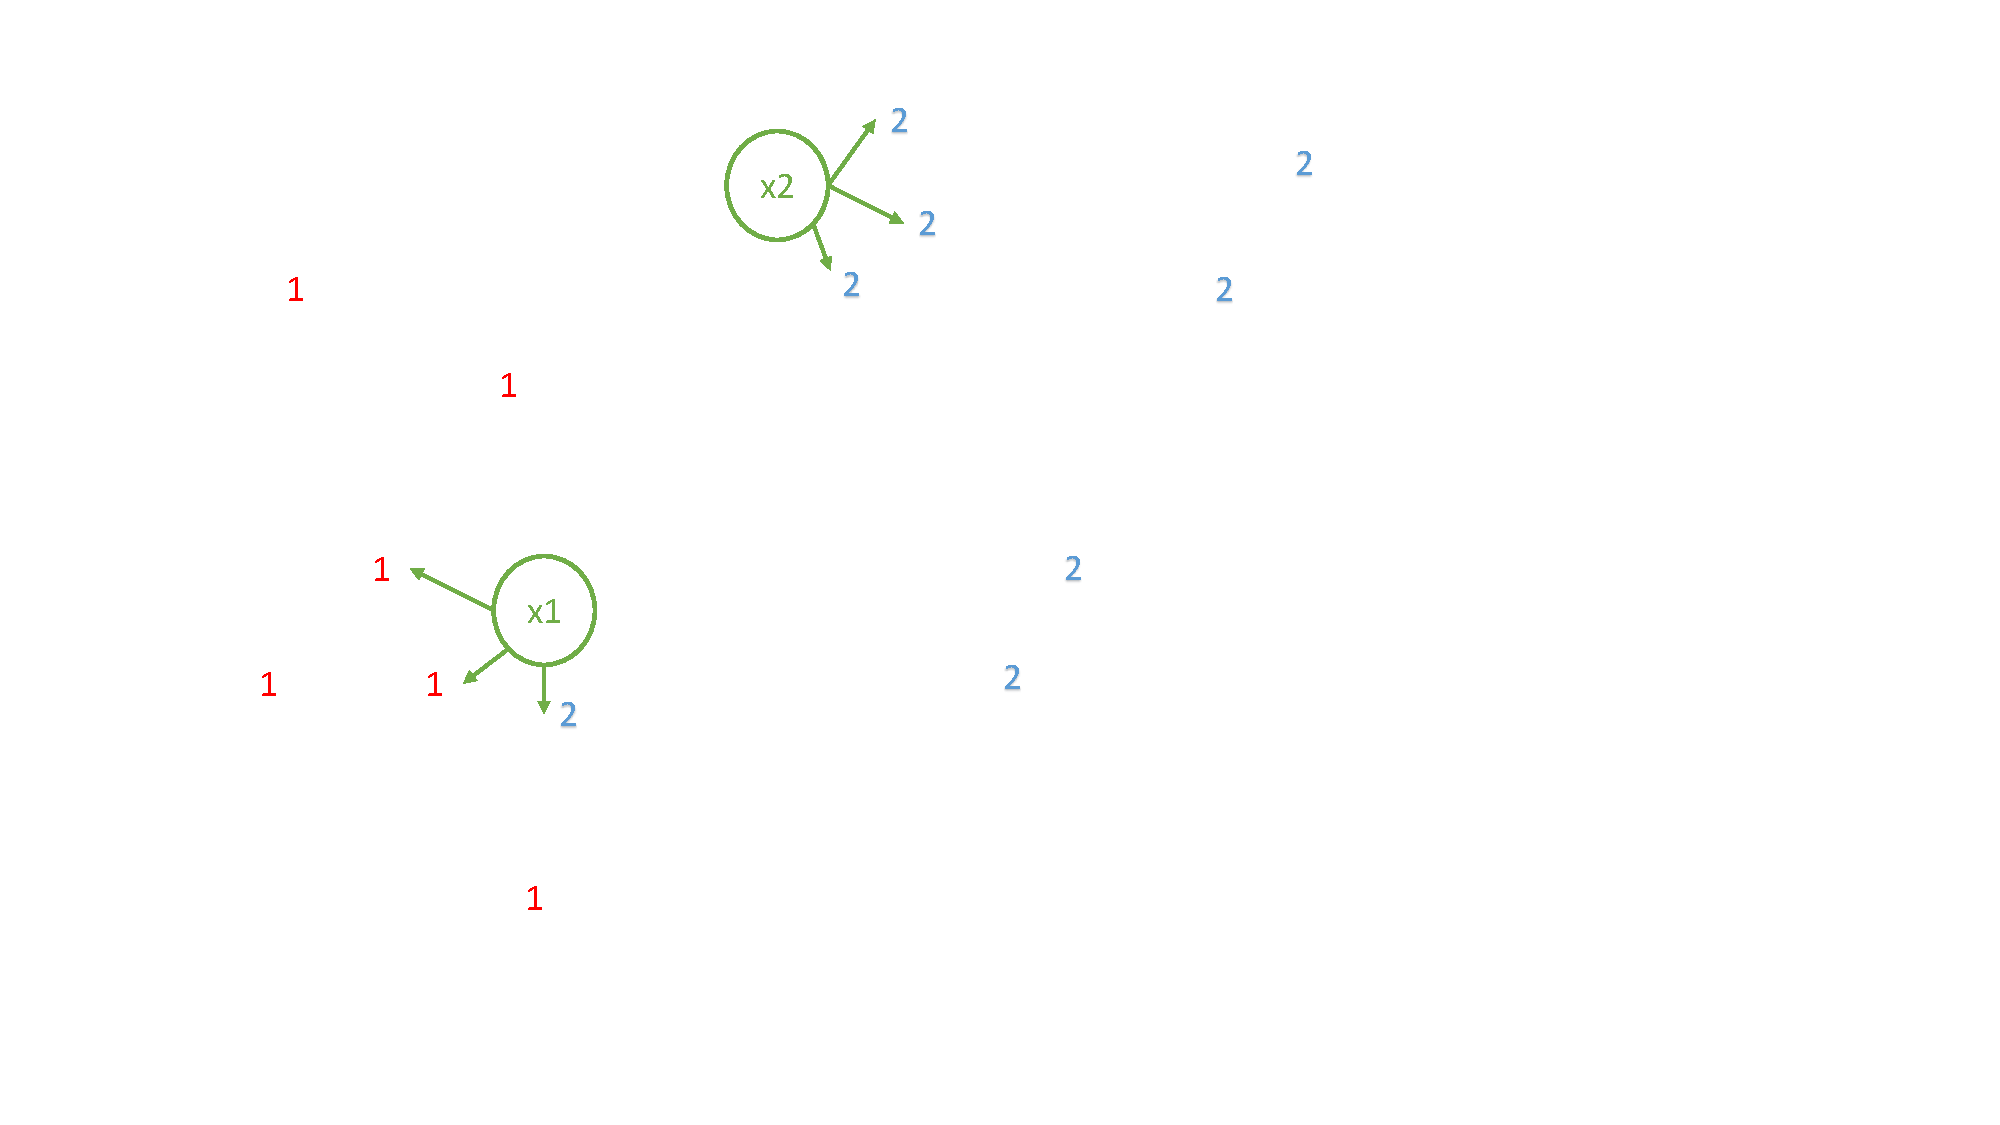
\includegraphics[width=0.49\textwidth]{classification.pdf}
	\caption{Geometric interpretation of the equidensity contours of the Gaussian.}
	\label{fig:example}
\end{figure}
Keep in mind that all the figures should be referred in text. For example, in Fig. \ref{fig:example} an example from the first lecture is shown.

\section{Exercise 3}
If you intend to present mathematical equations, please refer them properly in text. For example, the Fisher score is defined by (\ref{eq:fisher_score}).

\begin{equation}\label{eq:fisher_score}
    F = \displaystyle{\frac{\displaystyle{\sum _{j=1} ^ C p_j (\mu - \mu _j) ^2}}{\displaystyle{\sum _ {j=1} ^C} p_j \sigma _j ^2}}.
\end{equation}
In (\ref{eq:fisher_score}) $p_j$ denotes the fraction of points belonging to the class $j$. The mean values of the entire data set and the class $j$ are denoted by $\mu$ and $\mu _j$, respectively. Finally, $\sigma _j$ is the standard deviation within the class $j$. Hint: Do not waste space and time with the equations from the slides.
\section{Exercise 4}
Table environments can be complicated to learn, but allow one to save a lot of space in reporting the results.
\begin{table}[h]
\centering
\caption{Confusion matrix - Decision Tree Classifier}\label{tab:DT_confusion}.
\begin{tabular}{|l|c|c|}
\hline
{} &   Actual (PD) & Actual (HC) \\
\hline
Predicted (PD)         &  5 &      1 \\
\hline
Predicted (HC)         &  1 &      4 \\
\hline
\end{tabular}
\end{table}
Do not forget to refer to the Tab. \ref{tab:DT_confusion} in text.

\section{Exercise 5}
Please cite all the external sources you have used. As an example, this report is generated in \LaTeX \cite{latex2e}, which is based on \TeX{} described in\cite{texbook}. Do not cite lecture slides or the book by C. Aggarwal.

\section{Exercise 6}
Please follow the two-page limit for home assignment and the 4-page limit for the final project. Be creative and follow the guidelines. Good luck!
\bibliography{bibliography}

\end{document}
